\documentclass[ignorenonframetext,]{beamer}
\setbeamertemplate{caption}[numbered]
\setbeamertemplate{caption label separator}{:}
\setbeamercolor{caption name}{fg=normal text.fg}
\usepackage{amssymb,amsmath}
\usepackage{ifxetex,ifluatex}
\usepackage{fixltx2e} % provides \textsubscript
\usepackage{lmodern}
\ifxetex
  \usepackage{fontspec,xltxtra,xunicode}
  \defaultfontfeatures{Mapping=tex-text,Scale=MatchLowercase}
  \newcommand{\euro}{€}
\else
  \ifluatex
    \usepackage{fontspec}
    \defaultfontfeatures{Mapping=tex-text,Scale=MatchLowercase}
    \newcommand{\euro}{€}
  \else
    \usepackage[T1]{fontenc}
    \usepackage[utf8]{inputenc}
      \fi
\fi
% use upquote if available, for straight quotes in verbatim environments
\IfFileExists{upquote.sty}{\usepackage{upquote}}{}
% use microtype if available
\IfFileExists{microtype.sty}{\usepackage{microtype}}{}
\usepackage{color}
\usepackage{fancyvrb}
\newcommand{\VerbBar}{|}
\newcommand{\VERB}{\Verb[commandchars=\\\{\}]}
\DefineVerbatimEnvironment{Highlighting}{Verbatim}{commandchars=\\\{\}}
% Add ',fontsize=\small' for more characters per line
\usepackage{framed}
\definecolor{shadecolor}{RGB}{248,248,248}
\newenvironment{Shaded}{\begin{snugshade}}{\end{snugshade}}
\newcommand{\KeywordTok}[1]{\textcolor[rgb]{0.13,0.29,0.53}{\textbf{{#1}}}}
\newcommand{\DataTypeTok}[1]{\textcolor[rgb]{0.13,0.29,0.53}{{#1}}}
\newcommand{\DecValTok}[1]{\textcolor[rgb]{0.00,0.00,0.81}{{#1}}}
\newcommand{\BaseNTok}[1]{\textcolor[rgb]{0.00,0.00,0.81}{{#1}}}
\newcommand{\FloatTok}[1]{\textcolor[rgb]{0.00,0.00,0.81}{{#1}}}
\newcommand{\CharTok}[1]{\textcolor[rgb]{0.31,0.60,0.02}{{#1}}}
\newcommand{\StringTok}[1]{\textcolor[rgb]{0.31,0.60,0.02}{{#1}}}
\newcommand{\CommentTok}[1]{\textcolor[rgb]{0.56,0.35,0.01}{\textit{{#1}}}}
\newcommand{\OtherTok}[1]{\textcolor[rgb]{0.56,0.35,0.01}{{#1}}}
\newcommand{\AlertTok}[1]{\textcolor[rgb]{0.94,0.16,0.16}{{#1}}}
\newcommand{\FunctionTok}[1]{\textcolor[rgb]{0.00,0.00,0.00}{{#1}}}
\newcommand{\RegionMarkerTok}[1]{{#1}}
\newcommand{\ErrorTok}[1]{\textbf{{#1}}}
\newcommand{\NormalTok}[1]{{#1}}
\usepackage{url}
\usepackage{graphicx}
\makeatletter
\def\maxwidth{\ifdim\Gin@nat@width>\linewidth\linewidth\else\Gin@nat@width\fi}
\def\maxheight{\ifdim\Gin@nat@height>\textheight0.8\textheight\else\Gin@nat@height\fi}
\makeatother
% Scale images if necessary, so that they will not overflow the page
% margins by default, and it is still possible to overwrite the defaults
% using explicit options in \includegraphics[width, height, ...]{}
\setkeys{Gin}{width=\maxwidth,height=\maxheight,keepaspectratio}

% Comment these out if you don't want a slide with just the
% part/section/subsection/subsubsection title:
\AtBeginPart{
  \let\insertpartnumber\relax
  \let\partname\relax
  \frame{\partpage}
}
\AtBeginSection{
  \let\insertsectionnumber\relax
  \let\sectionname\relax
  \frame{\sectionpage}
}
\AtBeginSubsection{
  \let\insertsubsectionnumber\relax
  \let\subsectionname\relax
  \frame{\subsectionpage}
}

\setlength{\parindent}{0pt}
\setlength{\parskip}{6pt plus 2pt minus 1pt}
\setlength{\emergencystretch}{3em}  % prevent overfull lines
\setcounter{secnumdepth}{0}
\usepackage{lifecon}
\usepackage{url}

\title{Intro to the lifecontingencies R package}
\author{Giorgio Alfredo Spedicato, UnipolSai R\&D Ph.D C.Stat ACAS}
\date{19th April 2015}

\begin{document}
\frame{\titlepage}

\begin{frame}
\tableofcontents[hideallsubsections]
\end{frame}

\begin{frame}

\%\VignetteEngine{knitr::knitr}

\end{frame}

\begin{frame}{Intro}

\begin{itemize}[<+->]
\itemsep1pt\parskip0pt\parsep0pt
\item
  The lifecontingencies package (Spedicato 2013) will be introduced.
\item
  As first half 2015 it is the first R (Team 2012) package merging
  demographic and financial mathematics function in order to perform
  actuarial evaluation of life contingent insurances (annuities, life
  insurances, endowments, etc).
\item
  The applied examples will shown: how to load the R package, how to
  perform basic financial mathematics and demographic calculations, how
  to price and reserve financial products.
\end{itemize}

\end{frame}

\begin{frame}

\begin{itemize}[<+->]
\itemsep1pt\parskip0pt\parsep0pt
\item
  The final example will show how to mix lifecontingencies and
  demography (Rob J Hyndman et al. 2011) function to assess the
  mortality development impact on annuities.
\item
  The interested readers are suggested to look to the package's
  vignettes (also appeared in the Journal of Statistical Sofware) for a
  broader overview. (Dickson, Hardy, and Waters 2009; and Mazzoleni
  2000) provide and introduction of Actuarial Mathematics theory.
\item
  Also (Charpentier 2012) and (Charpentier 2014) discuss the software.
\end{itemize}

\end{frame}

\begin{frame}[fragile]{First moves into the lifecontingecies package}

\begin{block}{Loading the package}

\begin{itemize}[<+->]
\itemsep1pt\parskip0pt\parsep0pt
\item
  The package is loaded using
\end{itemize}

\begin{Shaded}
\begin{Highlighting}[]
\KeywordTok{library}\NormalTok{(lifecontingencies) }\CommentTok{#load the package}
\end{Highlighting}
\end{Shaded}

\begin{itemize}[<+->]
\itemsep1pt\parskip0pt\parsep0pt
\item
  It requires a recent version of R (\textgreater{}=3.0) and the
  markovchain package (Spedicato 2015). The development version of the
  package requires also Rcpp package (Eddelbuettel 2013).
\end{itemize}

\end{block}

\end{frame}

\begin{frame}[fragile]

\begin{block}{Financial mathematics}

\begin{itemize}[<+->]
\itemsep1pt\parskip0pt\parsep0pt
\item
  Actuarial mathematics calculation applies probability to quantify
  uncertainty on present values calculation.
\item
  Certain present value calculations can be directly evaluated by the
  package
\end{itemize}

\begin{Shaded}
\begin{Highlighting}[]
\NormalTok{capitals <-}\StringTok{ }\KeywordTok{c}\NormalTok{(-}\DecValTok{1000}\NormalTok{,}\DecValTok{200}\NormalTok{,}\DecValTok{500}\NormalTok{,}\DecValTok{700}\NormalTok{)}
\NormalTok{times <-}\StringTok{ }\KeywordTok{c}\NormalTok{(}\DecValTok{0}\NormalTok{,}\DecValTok{1}\NormalTok{,}\DecValTok{2}\NormalTok{,}\DecValTok{5}\NormalTok{)}
\CommentTok{#calculate a present value}
\KeywordTok{presentValue}\NormalTok{(}\DataTypeTok{cashFlows=}\NormalTok{capitals, }\DataTypeTok{timeIds=}\NormalTok{times, }
             \DataTypeTok{interestRates=}\FloatTok{0.03}\NormalTok{)}
\end{Highlighting}
\end{Shaded}

\begin{verbatim}
## [1] 269.2989
\end{verbatim}

\end{block}

\end{frame}

\begin{frame}[fragile]

\begin{itemize}[<+->]
\itemsep1pt\parskip0pt\parsep0pt
\item
  The presentValue function is the kernel of functions that are used to
  calculate annuities and accumulated values, also paid in fractional
  $k$ payments.
\end{itemize}

\begin{Shaded}
\begin{Highlighting}[]
\NormalTok{ann1 <-}\StringTok{ }\KeywordTok{annuity}\NormalTok{(}\DataTypeTok{i=}\FloatTok{0.03}\NormalTok{, }\DataTypeTok{n=}\DecValTok{5}\NormalTok{, }\DataTypeTok{k=}\DecValTok{1}\NormalTok{, }\DataTypeTok{type=}\StringTok{"immediate"}\NormalTok{)}
\NormalTok{ann2 <-}\StringTok{ }\KeywordTok{annuity}\NormalTok{(}\DataTypeTok{i=}\FloatTok{0.03}\NormalTok{, }\DataTypeTok{n=}\DecValTok{5}\NormalTok{, }\DataTypeTok{k=}\DecValTok{12}\NormalTok{, }\DataTypeTok{type=}\StringTok{"due"}\NormalTok{)}
\KeywordTok{c}\NormalTok{(ann1,ann2)}
\end{Highlighting}
\end{Shaded}

\begin{verbatim}
## [1] 4.579707 4.653791
\end{verbatim}

\end{frame}

\begin{frame}[fragile]

\begin{itemize}[<+->]
\item
  Such functions can be combined to price bonds and other classical
  financial products.
\item
  The following code exemplifies the calculation of a 5\% coupon bond at
  3\% yield rate when the term is ten year.
\end{itemize}

\begin{Shaded}
\begin{Highlighting}[]
\NormalTok{bondPrice<-}\DecValTok{5}\NormalTok{*}\KeywordTok{annuity}\NormalTok{(}\DataTypeTok{i=}\FloatTok{0.03}\NormalTok{,}\DataTypeTok{n=}\DecValTok{10}\NormalTok{)+}\DecValTok{100}\NormalTok{*}\FloatTok{1.03}\NormalTok{^-}\DecValTok{10}
\NormalTok{bondPrice}
\end{Highlighting}
\end{Shaded}

\begin{verbatim}
## [1] 117.0604
\end{verbatim}

\end{frame}

\begin{frame}[fragile]{Managing lifetables and actuarial tables}

\begin{itemize}[<+->]
\itemsep1pt\parskip0pt\parsep0pt
\item
  A lifetable object is an S4 class comprised by three slots: the age
  (from 0 to $\omega$), the people at risk at beginning of age x and the
  table name.
\end{itemize}

\begin{Shaded}
\begin{Highlighting}[]
\CommentTok{#create an demo lifetable}
\NormalTok{xDemo<-}\KeywordTok{seq}\NormalTok{(}\DataTypeTok{from=}\DecValTok{0}\NormalTok{,}\DataTypeTok{to=}\DecValTok{5}\NormalTok{,}\DataTypeTok{by=}\DecValTok{1}\NormalTok{)}
\NormalTok{lxDemo<-}\KeywordTok{c}\NormalTok{(}\DecValTok{100}\NormalTok{,}\DecValTok{95}\NormalTok{,}\DecValTok{90}\NormalTok{,}\DecValTok{60}\NormalTok{,}\DecValTok{30}\NormalTok{,}\DecValTok{5}\NormalTok{)}
\NormalTok{lifetableDemo<-}\KeywordTok{new}\NormalTok{(}\StringTok{"lifetable"}\NormalTok{,}\DataTypeTok{x=}\NormalTok{xDemo,}
                   \DataTypeTok{lx=}\NormalTok{lxDemo,}\DataTypeTok{name=}\StringTok{"Demo"}\NormalTok{)}
\end{Highlighting}
\end{Shaded}

\end{frame}

\begin{frame}[fragile]

\begin{itemize}[<+->]
\itemsep1pt\parskip0pt\parsep0pt
\item
  In practice, it is often more convenient to load an existing table
  from a CSV or XLS source. Some common tables have been bundled as
  data.frames within the package.
\item
  The example that follows creates the Italian IPS55 life table.
\end{itemize}

\begin{Shaded}
\begin{Highlighting}[]
\KeywordTok{data}\NormalTok{(demoIta) }\CommentTok{#using the internal Italian LT data set}
\NormalTok{lxIPS55M <-}\StringTok{ }\KeywordTok{with}\NormalTok{(demoIta, IPS55M)}
\CommentTok{#performing some fixings}
\NormalTok{pos2Remove <-}\StringTok{ }\KeywordTok{which}\NormalTok{(lxIPS55M %in%}\StringTok{ }\KeywordTok{c}\NormalTok{(}\DecValTok{0}\NormalTok{,}\OtherTok{NA}\NormalTok{))}
\NormalTok{lxIPS55M <-lxIPS55M[-pos2Remove]}
\NormalTok{xIPS55M <-}\KeywordTok{seq}\NormalTok{(}\DecValTok{0}\NormalTok{,}\KeywordTok{length}\NormalTok{(lxIPS55M)-}\DecValTok{1}\NormalTok{,}\DecValTok{1}\NormalTok{)}
\CommentTok{#creating the table}
\NormalTok{ips55M <-}\StringTok{ }\KeywordTok{new}\NormalTok{(}\StringTok{"lifetable"}\NormalTok{,}\DataTypeTok{x=}\NormalTok{xIPS55M, }
\DataTypeTok{lx=}\NormalTok{lxIPS55M,}\DataTypeTok{name=}\StringTok{"IPS 55 Males"}\NormalTok{)}
\end{Highlighting}
\end{Shaded}

\end{frame}

\begin{frame}[fragile]

\begin{itemize}[<+->]
\itemsep1pt\parskip0pt\parsep0pt
\item
  It is therefore easy to perform standard demographic calculations with
  the aid of package functions.
\end{itemize}

\begin{Shaded}
\begin{Highlighting}[]
\CommentTok{# decrements between age 65 and 70}
\KeywordTok{dxt}\NormalTok{(ips55M, }\DataTypeTok{x =} \DecValTok{65}\NormalTok{, }\DataTypeTok{t =} \DecValTok{5}\NormalTok{)}
\end{Highlighting}
\end{Shaded}

\begin{verbatim}
## [1] 3659.74
\end{verbatim}

\begin{Shaded}
\begin{Highlighting}[]
\CommentTok{# probabilities of death between age 80 and 85}
\KeywordTok{qxt}\NormalTok{(ips55M, }\DataTypeTok{x =} \DecValTok{80}\NormalTok{, }\DataTypeTok{t =} \DecValTok{2}\NormalTok{)}
\end{Highlighting}
\end{Shaded}

\begin{verbatim}
## [1] 0.07264833
\end{verbatim}

\begin{Shaded}
\begin{Highlighting}[]
\CommentTok{# expected curtate lifetime}
\KeywordTok{exn}\NormalTok{(ips55M, }\DataTypeTok{x =} \DecValTok{65}\NormalTok{)}
\end{Highlighting}
\end{Shaded}

\begin{verbatim}
## [1] 21.96873
\end{verbatim}

\end{frame}

\begin{frame}[fragile]{Pricing and reserving Life Contingent insurances}

\begin{itemize}[<+->]
\itemsep1pt\parskip0pt\parsep0pt
\item
  The pricing and reserving of pure endowments $\pureend{x}{n}$, term
  insurances, $\termins{x}{n}$, annuities $\ddot{a}_{x}^{\{m\}}$,
  endowments $\pureend{x}{n}$ can be easily handled within the package.
\item
  Performing such actuarial calculations requires to create an actuarial
  table (similar to a lifetable but with one more slot for the interest
  rate) that can be create as it is shown below.
\end{itemize}

\begin{Shaded}
\begin{Highlighting}[]
\CommentTok{#creates a new actuarial table}
\NormalTok{ips55Act<-}\KeywordTok{new}\NormalTok{(}\StringTok{"actuarialtable"}\NormalTok{,}
\DataTypeTok{x=}\NormalTok{ips55M@x,}\DataTypeTok{lx=}\NormalTok{ips55M@lx,}
\DataTypeTok{interest=}\FloatTok{0.02}\NormalTok{,}\DataTypeTok{name=}\StringTok{"IPS55M"}\NormalTok{)}
\end{Highlighting}
\end{Shaded}

\end{frame}

\begin{frame}[fragile]

\begin{itemize}[<+->]
\itemsep1pt\parskip0pt\parsep0pt
\item
  The example that follows computes the yearly premium
  $P=50000*\frac{\pureendc{30}{35}}{\anndue{30}{35}}$ for a pure
  endowment on 50K capital.
\end{itemize}

\begin{Shaded}
\begin{Highlighting}[]
\CommentTok{#compute APV}
\NormalTok{APV=}\FloatTok{50e3}\NormalTok{*}\KeywordTok{Exn}\NormalTok{(}\DataTypeTok{actuarialtable =} 
\NormalTok{ips55Act,}\DataTypeTok{x=}\DecValTok{30}\NormalTok{,}\DataTypeTok{n=}\DecValTok{35}\NormalTok{)}
\CommentTok{#compute Premium}
\NormalTok{P=APV/}\KeywordTok{axn}\NormalTok{(}\DataTypeTok{actuarialtable =}
\NormalTok{ips55Act,}\DataTypeTok{x=}\DecValTok{30}\NormalTok{,}\DataTypeTok{n=}\DecValTok{35}\NormalTok{)}
\KeywordTok{c}\NormalTok{(APV,P)}
\end{Highlighting}
\end{Shaded}

\begin{verbatim}
## [1] 23584.7564   938.1422
\end{verbatim}

\end{frame}

\begin{frame}[fragile]

\begin{itemize}[<+->]
\itemsep1pt\parskip0pt\parsep0pt
\item
  The package allows to easily perform sensitivities on the financials
  changing key parameters like term, interest, etc as we can see on a
  endowment purchased by a 30 years old policyholder for 30 years.
\end{itemize}

\begin{Shaded}
\begin{Highlighting}[]
\CommentTok{#defining the ranges}
\NormalTok{interest.range<-}\KeywordTok{seq}\NormalTok{(}\DataTypeTok{from=}\FloatTok{0.015}\NormalTok{, }\DataTypeTok{to=}\FloatTok{0.035}\NormalTok{,}\DataTypeTok{by=}\FloatTok{0.001}\NormalTok{)}
\NormalTok{term.range<-}\KeywordTok{seq}\NormalTok{(}\DataTypeTok{from=}\DecValTok{20}\NormalTok{, }\DataTypeTok{to=}\DecValTok{40}\NormalTok{,}\DataTypeTok{by=}\DecValTok{1}\NormalTok{)}
\CommentTok{#computing APV sensitivities}
\NormalTok{apv.interest.sensitivity<-}\KeywordTok{sapply}\NormalTok{(interest.range,}
\DataTypeTok{FUN =} \StringTok{"AExn"}\NormalTok{,}\DataTypeTok{actuarialtable=}\NormalTok{ips55Act,}\DataTypeTok{x=}\DecValTok{30}\NormalTok{,}\DataTypeTok{n=}\DecValTok{30}\NormalTok{)}
\NormalTok{apv.term.sensitivity<-}\KeywordTok{sapply}\NormalTok{(term.range,}\DataTypeTok{FUN =} \StringTok{"AExn"}\NormalTok{,}
                             \DataTypeTok{actuarialtable=}\NormalTok{ips55Act,}\DataTypeTok{x=}\DecValTok{30}\NormalTok{)}
\end{Highlighting}
\end{Shaded}

\end{frame}

\begin{frame}

\begin{itemize}[<+->]
\itemsep1pt\parskip0pt\parsep0pt
\item
  The graph below displays sensitivities on APV varying interest rate
  and insurance term.
\end{itemize}

\begin{center}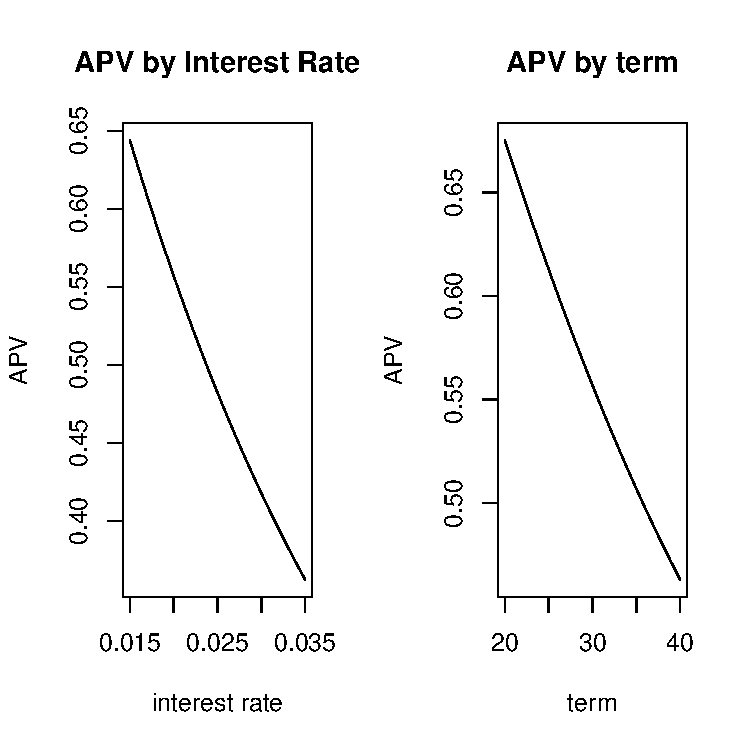
\includegraphics{introToLifecontingencies_files/figure-beamer/endowmentplot-1} \end{center}

\end{frame}

\begin{frame}[fragile]

\begin{itemize}[<+->]
\itemsep1pt\parskip0pt\parsep0pt
\item
  Also, calculation of outstanding reserves is made easy as the
  following example, applied on a 100K face value 40 year term term life
  insurance with payments made yearly on a policyholder aged 25, shows.
\end{itemize}

\begin{Shaded}
\begin{Highlighting}[]
\CommentTok{#compute the APV and premium}
\NormalTok{APV=}\FloatTok{100e3}\NormalTok{*}\KeywordTok{Axn}\NormalTok{(}\DataTypeTok{actuarialtable =} \NormalTok{ips55Act,}\DataTypeTok{x=}\DecValTok{25}\NormalTok{,}\DataTypeTok{n=}\DecValTok{40}\NormalTok{) }
\NormalTok{P=APV/}\KeywordTok{axn}\NormalTok{(}\DataTypeTok{actuarialtable =} \NormalTok{ips55Act,}\DataTypeTok{x=}\DecValTok{25}\NormalTok{,}\DataTypeTok{n=}\DecValTok{40}\NormalTok{)}
\CommentTok{#define a reserve function}
\NormalTok{reserveFunction<-function(t) }
  \FloatTok{100e3}\NormalTok{*}\KeywordTok{Axn}\NormalTok{(}\DataTypeTok{actuarialtable =} \NormalTok{ips55Act,}\DataTypeTok{x=}\DecValTok{25}\NormalTok{+t,}\DataTypeTok{n=}\DecValTok{40}\NormalTok{-t) -}\StringTok{ }
\StringTok{  }\NormalTok{P *}\KeywordTok{axn}\NormalTok{(}\DataTypeTok{actuarialtable =} \NormalTok{ips55Act,}\DataTypeTok{x=}\DecValTok{25}\NormalTok{+t,}\DataTypeTok{n=}\DecValTok{40}\NormalTok{-t)}
\NormalTok{reserve<-}\KeywordTok{sapply}\NormalTok{(}\DecValTok{0}\NormalTok{:}\DecValTok{40}\NormalTok{,reserveFunction)}
\end{Highlighting}
\end{Shaded}

\end{frame}

\begin{frame}

\begin{center}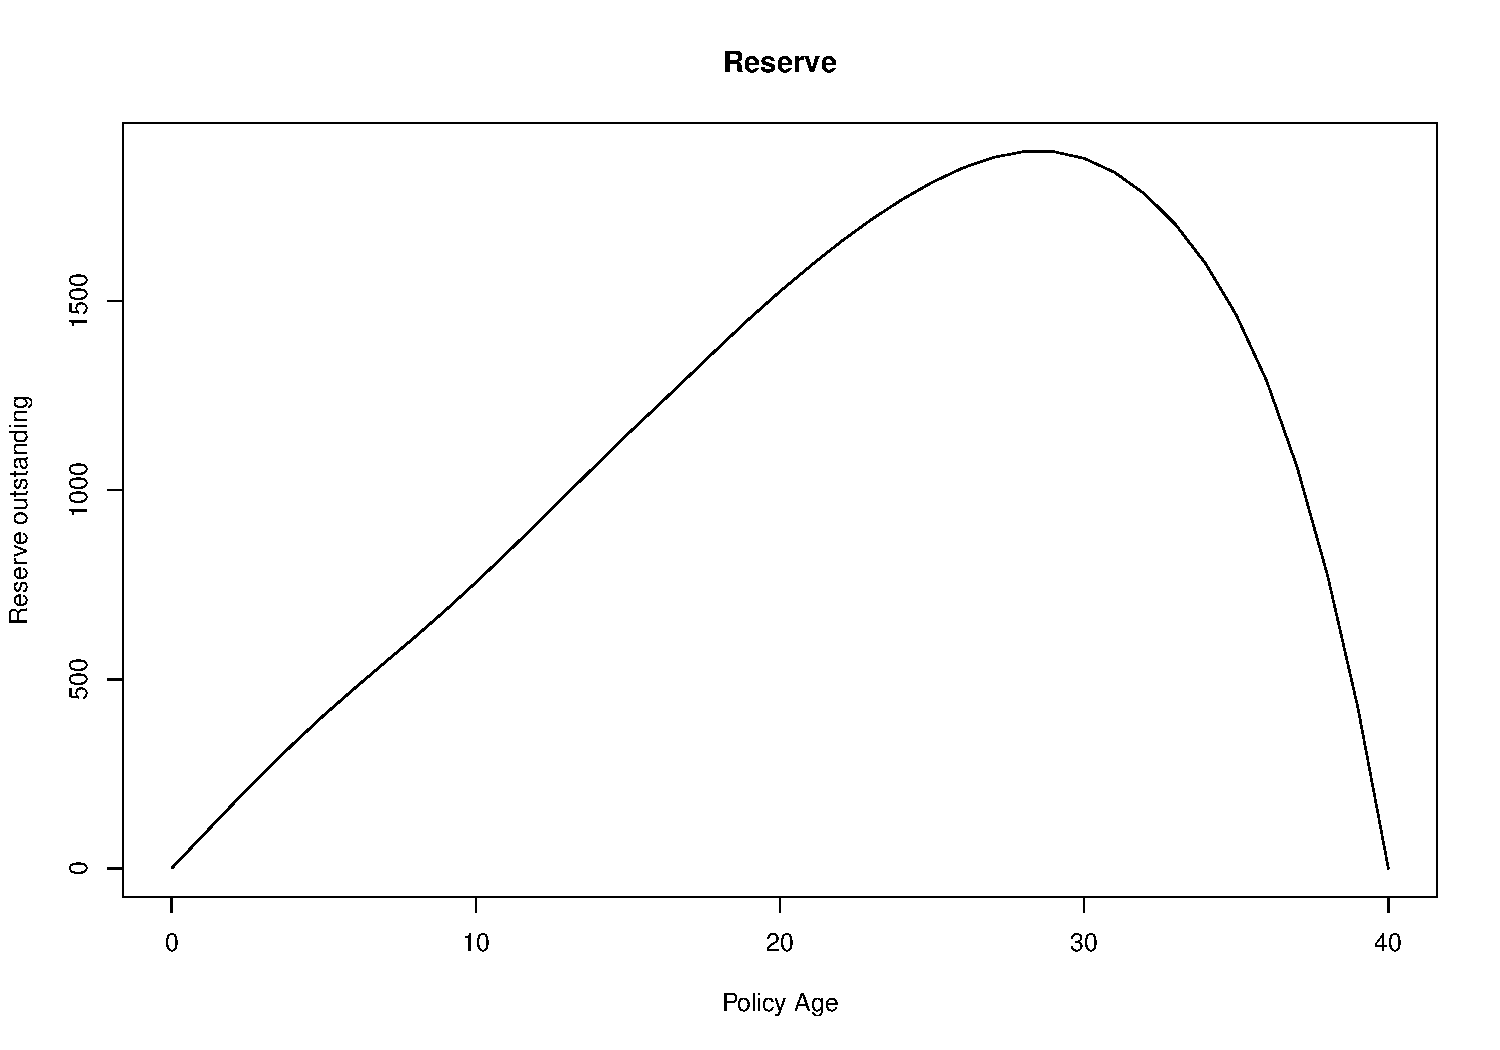
\includegraphics{introToLifecontingencies_files/figure-beamer/reserves2-1} \end{center}

\end{frame}

\begin{frame}[fragile]{Stochastic evalutation}

\begin{itemize}[<+->]
\itemsep1pt\parskip0pt\parsep0pt
\item
  The APV of a life contingent insurance is the expected value of a
  function of a random variable (the residual life time). Knowing the
  interest rate and the underlying life table it is possible both to
  compute the APV and to assess the distribution of the underlying life
  insurance.
\end{itemize}

\begin{Shaded}
\begin{Highlighting}[]
\CommentTok{#analyzing and Endowment of 100K on x=40, n=25}
\CommentTok{#compute APV}
\NormalTok{APV=}\KeywordTok{AExn}\NormalTok{(}\DataTypeTok{actuarialtable =} \NormalTok{ips55Act,}\DataTypeTok{x=}\DecValTok{40}\NormalTok{,}\DataTypeTok{n=}\DecValTok{25}\NormalTok{) }
\CommentTok{#sampling}
\NormalTok{AEXnDistr<-}\KeywordTok{rLifeContingencies}\NormalTok{(}\DataTypeTok{n=}\FloatTok{10e3}\NormalTok{,}
\DataTypeTok{lifecontingency =} \StringTok{"AExn"}\NormalTok{,}\DataTypeTok{x =} \DecValTok{40}\NormalTok{,}
\DataTypeTok{t=}\DecValTok{25}\NormalTok{,}\DataTypeTok{object =} \NormalTok{ips55Act)}
\end{Highlighting}
\end{Shaded}

\end{frame}

\begin{frame}[fragile]

\begin{itemize}[<+->]
\itemsep1pt\parskip0pt\parsep0pt
\item
  In order to assess if the distribution is unbiased we use a classical
  one sample t - test.
\end{itemize}

\begin{Shaded}
\begin{Highlighting}[]
\CommentTok{#assess if the expected value match the theoretical one}
\KeywordTok{t.test}\NormalTok{(}\DataTypeTok{x=}\NormalTok{AEXnDistr,}\DataTypeTok{mu =} \NormalTok{APV)}
\end{Highlighting}
\end{Shaded}

\begin{verbatim}
## 
##  One Sample t-test
## 
## data:  AEXnDistr
## t = -0.1688, df = 9999, p-value = 0.866
## alternative hypothesis: true mean is not equal to 0.6148635
## 95 percent confidence interval:
##  0.6141982 0.6154234
## sample estimates:
## mean of x 
## 0.6148108
\end{verbatim}

\end{frame}

\begin{frame}

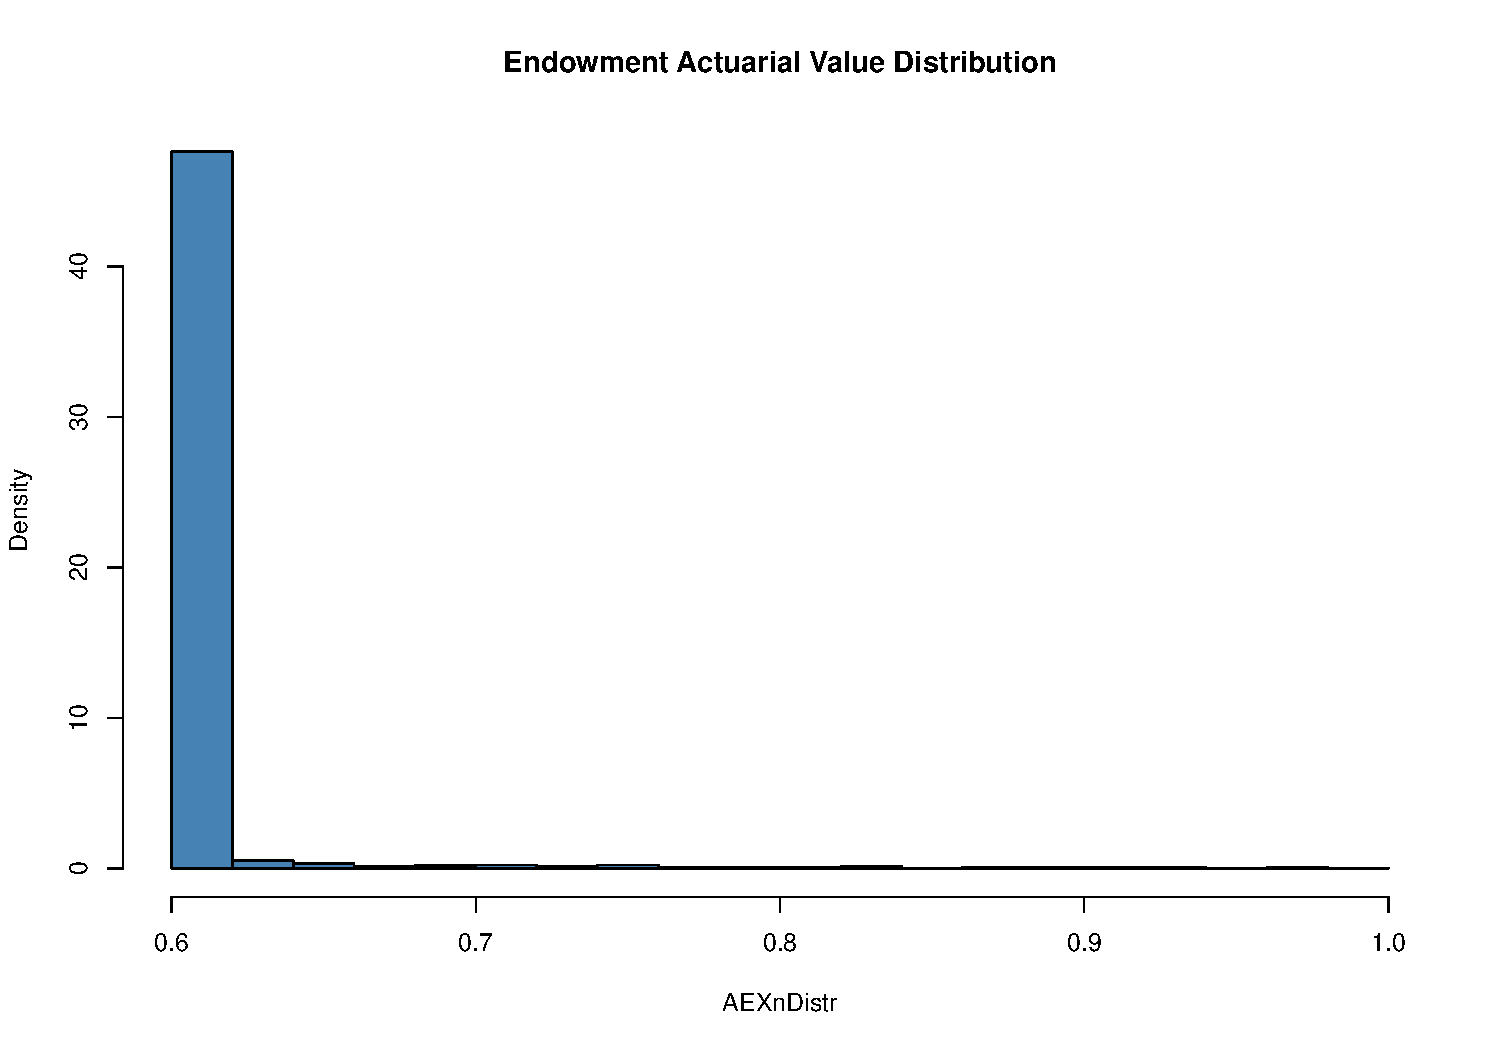
\includegraphics{introToLifecontingencies_files/figure-beamer/AEXn2-1.pdf}

\end{frame}

\begin{frame}[fragile]{Assessing longevity impact on annuities using
lifecontingencies and demography}

\begin{itemize}[<+->]
\itemsep1pt\parskip0pt\parsep0pt
\item
  This part of the presentation will make use of the demography package
  to calibrate Lee Carter (Lee and Carter 1992) model,
  $log\left(\mu_{x,t} \right) =a_{x}+b_{x}*k_{t}\rightarrow p_{x,t}=exp^{-\mu_{x,t}}$
  ,projecting mortality and implicit life tables.
\end{itemize}

\begin{Shaded}
\begin{Highlighting}[]
\CommentTok{#load the package and the italian tables}
\KeywordTok{library}\NormalTok{(demography) }
\CommentTok{#italy.demo<-hmd.mx("ITA", username="yourUN", }
\CommentTok{#password="yourPW")}
\KeywordTok{load}\NormalTok{(}\DataTypeTok{file=}\StringTok{"mortalityDatasets.RData"}\NormalTok{) }\CommentTok{#load the dataset}
\end{Highlighting}
\end{Shaded}

\end{frame}

\begin{frame}[fragile]

\begin{itemize}[<+->]
\itemsep1pt\parskip0pt\parsep0pt
\item
  Lee Carter model is calibrated using lca function.
\item
  Then an arima model is used to project (extrapolate) the underlying
  $k_t$ over the historical period.
\end{itemize}

\begin{Shaded}
\begin{Highlighting}[]
\CommentTok{#calibrate lee carter}
\NormalTok{italy.leecarter<-}\KeywordTok{lca}\NormalTok{(}\DataTypeTok{data=}\NormalTok{italyDemo,}\DataTypeTok{series=}\StringTok{"total"}\NormalTok{,}
                     \DataTypeTok{max.age=}\DecValTok{103}\NormalTok{,}\DataTypeTok{adjust =} \StringTok{"none"}\NormalTok{)}
\CommentTok{#perform modeling of kt series}
\NormalTok{kt.model<-}\KeywordTok{auto.arima}\NormalTok{(italy.leecarter$kt)}
\CommentTok{#projecting the kt}
\NormalTok{kt.forecast<-}\KeywordTok{forecast}\NormalTok{(kt.model,}\DataTypeTok{h=}\DecValTok{100}\NormalTok{) }
\end{Highlighting}
\end{Shaded}

\end{frame}

\begin{frame}[fragile]

-The code below generates the matrix of prospective life tables

\begin{Shaded}
\begin{Highlighting}[]
\CommentTok{#indexing the kt}
\NormalTok{kt.full<-}\KeywordTok{ts}\NormalTok{(}\KeywordTok{union}\NormalTok{(italy.leecarter$kt, kt.forecast$mean),}
            \DataTypeTok{start=}\DecValTok{1872}\NormalTok{)  }
\CommentTok{#getting and defining the life tables matrix}
\NormalTok{mortalityTable<-}\KeywordTok{exp}\NormalTok{(italy.leecarter$ax}
\NormalTok{+italy.leecarter$bx%*%}\KeywordTok{t}\NormalTok{(kt.full)) }
\KeywordTok{rownames}\NormalTok{(mortalityTable)<-}\KeywordTok{seq}\NormalTok{(}\DataTypeTok{from=}\DecValTok{0}\NormalTok{, }\DataTypeTok{to=}\DecValTok{103}\NormalTok{)}
\KeywordTok{colnames}\NormalTok{(mortalityTable)<-}\KeywordTok{seq}\NormalTok{(}\DataTypeTok{from=}\DecValTok{1872}\NormalTok{, }
\DataTypeTok{to=}\DecValTok{1872}\NormalTok{+}\KeywordTok{dim}\NormalTok{(mortalityTable)[}\DecValTok{2}\NormalTok{]-}\DecValTok{1}\NormalTok{)}
\end{Highlighting}
\end{Shaded}

\end{frame}

\begin{frame}

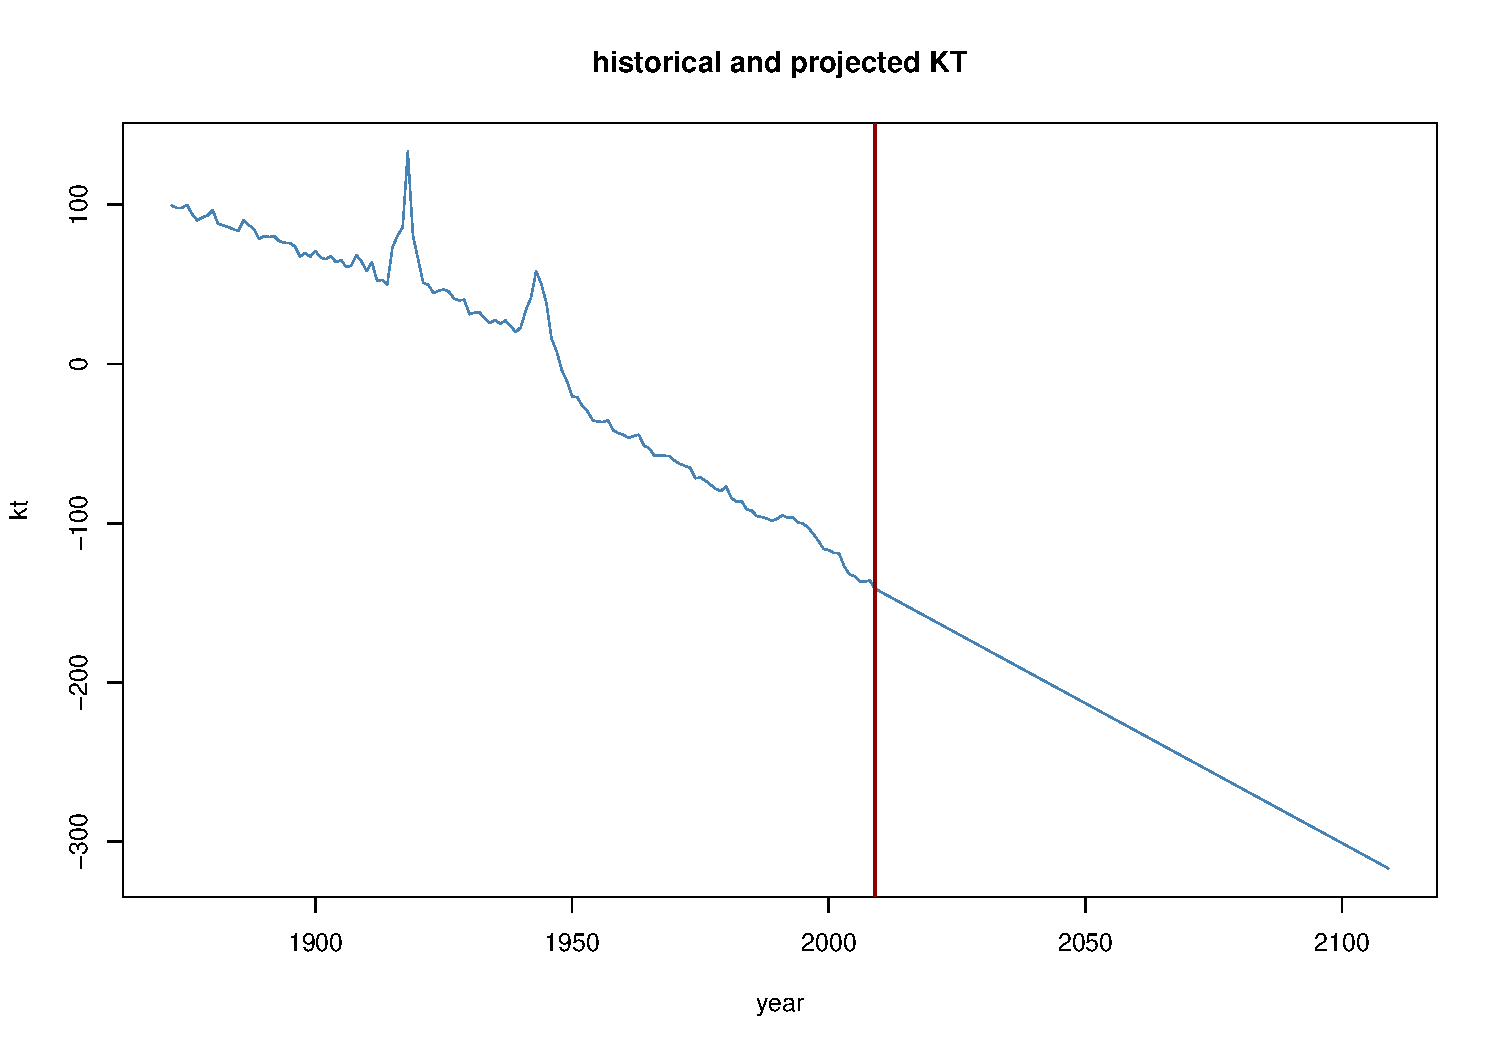
\includegraphics{introToLifecontingencies_files/figure-beamer/leecarter2plot-1.pdf}

\end{frame}

\begin{frame}[fragile]

\begin{itemize}[<+->]
\itemsep1pt\parskip0pt\parsep0pt
\item
  now we need a function that returns the one-year death probabilities
  given a year of birth (cohort.
\end{itemize}

\begin{Shaded}
\begin{Highlighting}[]
\NormalTok{getCohortQx<-function(yearOfBirth)}
\NormalTok{\{}
  \NormalTok{colIndex<-}\KeywordTok{which}\NormalTok{(}\KeywordTok{colnames}\NormalTok{(mortalityTable)}
                  \NormalTok{==yearOfBirth) }\CommentTok{#identify }
  \CommentTok{#the column corresponding to the cohort }
  \CommentTok{#definex the probabilities from which }
  \CommentTok{#the projection is to be taken}
  \NormalTok{maxLength<-}\KeywordTok{min}\NormalTok{(}\KeywordTok{nrow}\NormalTok{(mortalityTable)-}\DecValTok{1}\NormalTok{,}
                 \KeywordTok{ncol}\NormalTok{(mortalityTable)-colIndex)}
  \NormalTok{qxOut<-}\KeywordTok{numeric}\NormalTok{(maxLength}\DecValTok{+1}\NormalTok{)}
  \NormalTok{for(i in }\DecValTok{0}\NormalTok{:maxLength)}
    \NormalTok{qxOut[i}\DecValTok{+1}\NormalTok{]<-mortalityTable[i}\DecValTok{+1}\NormalTok{,colIndex+i]}
  \CommentTok{#fix: we add a fictional omega age where }
  \CommentTok{#death probability = 1}
  \NormalTok{qxOut<-}\KeywordTok{c}\NormalTok{(qxOut,}\DecValTok{1}\NormalTok{)}
  \KeywordTok{return}\NormalTok{(qxOut)}
\NormalTok{\}}
\end{Highlighting}
\end{Shaded}

\end{frame}

\begin{frame}[fragile]

\begin{itemize}[<+->]
\itemsep1pt\parskip0pt\parsep0pt
\item
  Now we use such function to obtain prospective life tables and to
  perform actuarial calculations. For example, we can compute the APV of
  an annuity on a workers' retiring at 65 assuming he were born in 1920,
  in 1950 and in 1980. We will use the interest rate of 1.5\% (the one
  used to compute Italian Social Security annuity factors).
\item
  The first step is to generate the life and actuarial tables
\end{itemize}

\begin{Shaded}
\begin{Highlighting}[]
\CommentTok{#generate the life tables}
\NormalTok{qx1920<-}\KeywordTok{getCohortQx}\NormalTok{(}\DataTypeTok{yearOfBirth =} \DecValTok{1920}\NormalTok{)}
\NormalTok{lt1920<-}\KeywordTok{probs2lifetable}\NormalTok{(}\DataTypeTok{probs=}\NormalTok{qx1920,}\DataTypeTok{type=}\StringTok{"qx"}\NormalTok{,}
\DataTypeTok{name=}\StringTok{"Table 1920"}\NormalTok{)}
\NormalTok{at1920<-}\KeywordTok{new}\NormalTok{(}\StringTok{"actuarialtable"}\NormalTok{,}\DataTypeTok{x=}\NormalTok{lt1920@x,}
\DataTypeTok{lx=}\NormalTok{lt1920@lx,}\DataTypeTok{interest=}\FloatTok{0.015}\NormalTok{)}
\NormalTok{qx1950<-}\KeywordTok{getCohortQx}\NormalTok{(}\DataTypeTok{yearOfBirth =} \DecValTok{1950}\NormalTok{)}
\NormalTok{lt1950<-}\KeywordTok{probs2lifetable}\NormalTok{(}\DataTypeTok{probs=}\NormalTok{qx1950,}
\DataTypeTok{type=}\StringTok{"qx"}\NormalTok{,}\DataTypeTok{name=}\StringTok{"Table 1950"}\NormalTok{)}
\NormalTok{at1950<-}\KeywordTok{new}\NormalTok{(}\StringTok{"actuarialtable"}\NormalTok{,}\DataTypeTok{x=}\NormalTok{lt1950@x,}
\DataTypeTok{lx=}\NormalTok{lt1950@lx,}\DataTypeTok{interest=}\FloatTok{0.015}\NormalTok{)}
\NormalTok{qx1980<-}\KeywordTok{getCohortQx}\NormalTok{(}\DataTypeTok{yearOfBirth =} \DecValTok{1980}\NormalTok{)}
\NormalTok{lt1980<-}\KeywordTok{probs2lifetable}\NormalTok{(}\DataTypeTok{probs=}\NormalTok{qx1980,}
\DataTypeTok{type=}\StringTok{"qx"}\NormalTok{,}\DataTypeTok{name=}\StringTok{"Table 1980"}\NormalTok{)}
\NormalTok{at1980<-}\KeywordTok{new}\NormalTok{(}\StringTok{"actuarialtable"}\NormalTok{,}\DataTypeTok{x=}\NormalTok{lt1980@x,}
\DataTypeTok{lx=}\NormalTok{lt1980@lx,}\DataTypeTok{interest=}\FloatTok{0.015}\NormalTok{)}
\end{Highlighting}
\end{Shaded}

\end{frame}

\begin{frame}[fragile]

\begin{itemize}[<+->]
\itemsep1pt\parskip0pt\parsep0pt
\item
  Now we can evaluate $\ddot{a}_{65}$ and $\mathring{e}_{65}$ for
  workers born in 1920, 1950 and 1980 respectively.
\end{itemize}

\begin{Shaded}
\begin{Highlighting}[]
\KeywordTok{cat}\NormalTok{(}\StringTok{"Results for 1920 cohort"}\NormalTok{,}\StringTok{"}\CharTok{\textbackslash{}n}\StringTok{"}\NormalTok{)}
\end{Highlighting}
\end{Shaded}

\begin{verbatim}
## Results for 1920 cohort
\end{verbatim}

\begin{Shaded}
\begin{Highlighting}[]
\KeywordTok{c}\NormalTok{(}\KeywordTok{exn}\NormalTok{(at1920,}\DataTypeTok{x=}\DecValTok{65}\NormalTok{),}\KeywordTok{axn}\NormalTok{(at1920,}\DataTypeTok{x=}\DecValTok{65}\NormalTok{))}
\end{Highlighting}
\end{Shaded}

\begin{verbatim}
## [1] 16.51391 15.14127
\end{verbatim}

\begin{Shaded}
\begin{Highlighting}[]
\KeywordTok{cat}\NormalTok{(}\StringTok{"Results for 1950 cohort"}\NormalTok{,}\StringTok{"}\CharTok{\textbackslash{}n}\StringTok{"}\NormalTok{)}
\end{Highlighting}
\end{Shaded}

\begin{verbatim}
## Results for 1950 cohort
\end{verbatim}

\begin{Shaded}
\begin{Highlighting}[]
\KeywordTok{c}\NormalTok{(}\KeywordTok{exn}\NormalTok{(at1950,}\DataTypeTok{x=}\DecValTok{65}\NormalTok{),}\KeywordTok{axn}\NormalTok{(at1950,}\DataTypeTok{x=}\DecValTok{65}\NormalTok{))}
\end{Highlighting}
\end{Shaded}

\begin{verbatim}
## [1] 18.72669 16.83391
\end{verbatim}

\begin{Shaded}
\begin{Highlighting}[]
\KeywordTok{cat}\NormalTok{(}\StringTok{"Results for 1980 cohort"}\NormalTok{,}\StringTok{"}\CharTok{\textbackslash{}n}\StringTok{"}\NormalTok{)}
\end{Highlighting}
\end{Shaded}

\begin{verbatim}
## Results for 1980 cohort
\end{verbatim}

\begin{Shaded}
\begin{Highlighting}[]
\KeywordTok{c}\NormalTok{(}\KeywordTok{exn}\NormalTok{(at1980,}\DataTypeTok{x=}\DecValTok{65}\NormalTok{),}\KeywordTok{axn}\NormalTok{(at1980,}\DataTypeTok{x=}\DecValTok{65}\NormalTok{))}
\end{Highlighting}
\end{Shaded}

\begin{verbatim}
## [1] 20.47112 18.13948
\end{verbatim}

\end{frame}

\begin{frame}[allowframebreaks]{Bibliography}

Charpentier, Arthur. 2012. ``Actuarial Science with R 2: Life Insurance
and Mortality Tables.''
\url{http://freakonometrics.blog.free.fr/index.php?post/2012/04/04/Life-insurance,-with-R,-Meielisalp}.

---------. 2014. \emph{Computational Actuarial Science}. The R Series.
Cambridge University Press.

Dickson, D.C.M., M.R. Hardy, and H.R. Waters. 2009. \emph{Actuarial
Mathematics for Life Contingent Risks}. International Series on
Actuarial Science. Cambridge University Press.

Eddelbuettel, Dirk. 2013. \emph{Seamless R and C++ Integration with
Rcpp}. New York: Springer.

Lee, R.D., and L.R. Carter. 1992. ``Modeling and Forecasting U.S.
Mortality.'' \emph{Journal of the American Statistical Association} 87
(419): 659--75.
doi:\href{http://dx.doi.org/10.2307/2290201}{10.2307/2290201}.

Mazzoleni, P. 2000. \emph{Appunti Di Matematica Attuariale}. EDUCatt
Università Cattolica.

Rob J Hyndman, Heather Booth, Leonie Tickle, and John Maindonald. 2011.
\emph{demography: Forecasting Mortality, Fertility, Migration and
Population Data}. \url{http://CRAN.R-project.org/package=demography}.

Spedicato, Giorgio Alfredo. 2013. ``The lifecontingencies Package:
Performing Financial and Actuarial Mathematics Calculations in R.''
\emph{Journal of Statistical Software} 55 (10): 1--36.
\url{http://www.jstatsoft.org/v55/i10/}.

---------. 2015. \emph{markovchain: discrete Time Markov Chains Made
Easy}.

Team, R Development Core. 2012. \emph{R: A Language and Environment for
Statistical Computing}. Vienna, Austria: R Foundation for Statistical
Computing. \url{http://www.R-project.org/}.

\end{frame}

\end{document}
